\documentclass[10pt]{article}

\usepackage{amsmath}
\usepackage{amssymb}
\usepackage{graphicx}
%\usepackage{picins}
\usepackage{amsthm}
\usepackage{bbm}

\setlength{\voffset}{-28.4mm}
\setlength{\hoffset}{-1in}
\setlength{\topmargin}{20mm}
\setlength{\oddsidemargin}{25mm}
\setlength{\evensidemargin}{25mm}
\setlength{\textwidth}{160mm}
\usepackage{subfigure}

\setlength{\parindent}{0pt}

\setlength{\textheight}{235mm}
%\setlength{\footskip}{20mm}
\setlength{\headsep}{50pt}
\setlength{\headheight}{0pt}

% Paket zur Verwendung einer verbesserten Schriftart
\usepackage{lmodern}

%Language package französisch
\usepackage[english]{babel}
\usepackage[T1]{fontenc}
\usepackage[utf8]{inputenc}


%Hyperref
\usepackage[backref = true]{hyperref}

\begin{document}
	
\title{Recherche rapide d’un triangle contenant un point dans un maillage}

\section{}

R3: $<,>,<=,>=$\\
ordre lexicographie sur les pair est deja dans la stl

\subsection{Multimaps}
(Requires a less-than comparison function.)\\

$ O(3 n_T)$: jede Kante jedes Dreiecks als Schlüssel\\
$|K| \ O(log(n_T)):$ Zugriff auf Container fur jede Kante\\
$\Rightarrow O(n_T log(n_T))$\\
speichern in 2dim Array: Zugriff in konstanter Zeit\\

\textbf{unordered map}(hash tables) has constant time performance on all operations provided no collisions occur. When collisions occur, traversal of a linked list containing all elements of the same bucket (those that hash to the same value) is necessary, and in the worst case, there is only one bucket; hence O(n)\\

\subsection{Listen}

$ O(3 n_T)$, push front(): jede Kante jedes Dreiecks einfügen\\
$ O(N logN)$, container size $N$: sort(): definiere hierfür $<$ für R3 (Nach ersten und dann nach zweitem Element sortieren etc)\\

\textbf{doppelt verlinkt! und dann mit Kante und Sommet prev und next von Listenelement!}\\
konstanter Zugriff mit Iterator!\\

$ O(3 n_T)$: pop front und speichern in 2 dim array\\

Alternative für 2D array für konstanten Zugriff?\\
Daten könnten direkt in 2D array gespeichert werden, Listen und Maps überflüssig\\

\subsection{aire}

orientierter Flächeninhalt
$$ (a_i,b_i,p) = (a_i \times b_i ) \cdot p = \det(a_i,b_i,p) $$
bei det Vektoren in Zeilen


\newpage

\section{Première tentative de documentation}

\section{Le projet}

\section{La classe template T3 et la classe Triangle}

Objects of the class T3 represent elements of a three dimensional space in T. Hereby, the data type T is defined using a template. Within this project, either $T3<int>$ for the definition of a triangle (see \ref{triangle}) or $T3<double>$ for the definition of the coordinates of a vertex (see X) is used. The private members $x,y$ and $z$ store the entries of the T3 vector. The class has a default constructor, a constructor by copy and a constructor creating a vector given the three vector entries. Moreover, the class has operators to access and modify the entries (private), add to elements of T3, multiply an element of T3 by a scalar of the type T and calculate the scalar product of two T3 vectors. The operator $<$ compares two elements of T3 in the following way XXX. This allows a lexicographic ordering of a list of T3 elements (see \ref{list}, $T3<int>$). Given three T3 vectors, the method $ oriented_vol $ computes the signed volume of the triangles with vertices given by the input vectors. The sign is positive for triangles oriented in trigonometric sense. This method is used to \\
promenade \ref{promenade}, in desired direction \\


\subsection{The class triangle} \label{triangle}
The class triangle inherits form the class T3. Its derived members $ x,y,z $ are specialized as integers representing the position of its defining vertices in the array of the points of the given mesh. This array is a member of the class mesh (SHOULD be changed from maillage to mesh...) in \ref{mesh}. In addition, it has three extra integer members {\itshape neighbor1, neighbor2, neighbor3} representing the position of the adjacent triangles in the array of triangles which is also a member of the class mesh. An adjacent triangle $ t^{'} $ is said to be  {\itshape neighbor1 } of a triangle $ t $ if $ x $ is the first vertex of $t$ and $x$ is not a vertex of $ t^{'} $. The same holds for the indices $ 2,3 $. Note that this relation is not symmetric, that is to say that $ t^{'} $ is {\itshape neighbor1} does not imply that $t$ is {\itshape neighbor1} of $t^{'}$. 
Note that this assignment facilitates the access to the following in the algorithm {\itshape promenade} (see \ref{}).  \\
At the creation of a new triangle the latter three members are initialized by $ -1 $ which means that a triangle has no neighbors when it is created. The neighbors are set via the functions {\itshape setAdjacencyViaMultimap} \ref{multimap}, respectively {\itshape setAdjacencyViaList} \ref{list}. After the execution of one of these two functions $neighbor1 =  -1 $ describes the case that there is no adjacent triangle on the opposite side of the first vertex. 
Since the neighbors are private members there are getter and setter in order to read and manipulate them. \\



\section{The class mesh} \label{mesh}
The class mesh contains all necessary information of the mesh and the search of a point in (or outside) the mesh can be realized by its member functions. Its private members are pointers to the arrays of points and triangles of the mesh as integers who store the size of these two lists.
In order to create an object of type mesh the name of the desired .msh file has to be transmitted. The file is read by the functions {\itshape LoadNodes} and {\itshape LoadTriangles} \ref{Load} who then initialize the members {\itshape triangles, sommets, numbTriangles, numbSommets}. 
There are getter and setter for {\itshape numbTriangles, numbSommets} as well as getter for {\itshape triangles, sommets}. The functions {\itshape LoadTriangles, LoadNodes} are their setters. 


\subsection{LoadNodes and LoadTriangles} \label{Load}
Both functions are called in the constructor of the class mesh setting the members {\itshape nodes (VERTICES??)} and {\itshape triangles}. 
They work basically the same way with the small difference that they create arrays of different data types and searching for different key words in the .msh file. 
At first the .msh file is opened according to its name. Then the functions search for the line indicating the number of nodes respectively the number of triangles. 
To make the code work the next line must include the according number which is then stored in {\itshape numbSommets}, respectively {\itshape numbTri}. The data is read as a string which is transformed to an integer by the command {\itshape astoi}. These numbers also define the size of the arrays of $  type T3<double> $ and Triangle which are created by new. The following lines must include the coordinates of all nodes, respectively the positions of the triangles in the table of nodes. The lines are read as strings who are then 
Both functions finally return the arrays filled with the according nodes or triangles. 


\newpage

Adj vis Map, Exp Gnu

O Prom, Adj vis List, find Sommets und Rec



\subsection{Find the adjacent triangle}

\subsubsection{setAdjacencyViaMultimap} \label{multimap}

The goal of this function is the initialization of the members {\itshape neighbor1, neighbor2, neighbor3} of the class triangle. As a reminder they are defined by their position in the array of triangles. Their initialization is realized by the container {\itshape multimaps}. 
Each triangle $ t = (v_{i_1},v_{i_2},v_{i_3}) $ is represented by the sequence $ (i_1,i_2,i_3) $ where these indices indicate the position of the vertices in the array of vertices. 
For each $ t $ three pairs are added to the multimap, where the edges $(v_{i_k},v_{i_l}), \, k,l \in \{1,2,3\}, \ k \neq l $, stored by the data type $ pair<int,int> $ (more precisely $ pair<k,l> $), represent the keys, whereas the mapped value is an integer representing the position of the triangle in the array of triangles. Hence the initalization if the mulimap is realized in $ 3n_T $ loops, so in $ O(n_T) $. \\
Essentially for the functioning of the method is the ordering of the of the indices $ i_1,i_2,i_3 $ in $ t $. As in {\itshape setAdjacencyViaList} an edge $ \{ v_k, v_l\} $
 has to be uniquely identified by the pair $ (k,l) $ which should not be mixed up with $(l,k) $. This is achieved by demanding that for each triangle $ t =  (v_{i_1},v_{i_2},v_{i_3})$ the vertices are ordered, so $ i_1 < i_2 < i_3 $. Thus, an edge $(v_{i_k},v_{i_l}) $ can uniquely be identified by the pair $ (k,l), \, k < l $. \\
 We find the adjacent triangles by the following three steps: 
 \begin{enumerate}
 	\item 
 	We range over the multimap and in each step we save the key $ (i_k,i_l) $ and the associated position $ i $ of th triangle $ t = (v_{i_1},v_{i_2},v_{i_3})  $. Then we erase the element $ ( (i_k,i_l), \, i) $ of the multimap which is realized in constant time. 
 	\item 
 	Now searching by the function $ find $ for the stored key $ (i_k,i_l) $ allows us to determine if there is another index $ j $ associated to $ (i_k,i_l) $. If this is the case (the iterator returned by find does not point to the last element of the multimap) the triangles represented by $i$ and $j$ are adjacent. The function  $ find $ needs $ O(\log(n_T)) $ in order to return an iterator. 
 	Note that the pair $ ( (i_k,i_l), \, j) $ is not erased. This would yield an error because the actual iterator would try to access that element. 
 	\item 
 	The indices $ i $ and $ j $ are set as the neighbors of each other where $ j $ is set as neighbor $ k \in \{1,2,3\} $ if the index $k$ does not represent a vertex of the triangle represented by $ j $. The same rule is applied to $ i $ as a neighbor of $ j $. 
 	This assignment is realized in constant time. 
  \end{enumerate}
The application of all three steps needs a time of $ O(n_T)O(\log(n_T)) = O(n\log(n_T)) $. 




\subsubsection{setAdjacencyViaList} \label{list}
As in setAdjacencyViaMultimap, this method sets the members, describing the neighbors, for each triangle in the considered mesh. In the same manner as before, the members are described using their position in the triangle array.

The idea is to store each triangle, in varying order, three times in a list. For the triangle $t$ with the points $(a_1,a_2,a_3)$, the triangles $(a_1,a_2,t), (a_1,a_3,t)$ and $(a_2,a_3,t)$ are appended to the list. The creation of this list has complexity $O(3n_T)$.

After the creation, the list is sorted in lexicographic order. The complexity for sorting a list with $n_T$ elements is $O(n_Tlogn_T)$.

Due to the lexicographical ordering, the list allows now to define adjacencies between triangles. Two consecutive triangles of the list are considered. The first two entries of the triangles are compared. If they are equal, the triangles share an edge and can be defined as adjacent. $(a,b,t_1), (a,b,t_2)$

complexity $O(3n_T)$

In summary, the method setAdjacencyViaList has complexity $O(n_Tlogn_T)$.

Laufzeitvergleich

\subsection{L'algorithme promenade} \label{promenade}
$
min_neg random_neg
$

\begin{figure}[h]
	\subfigure{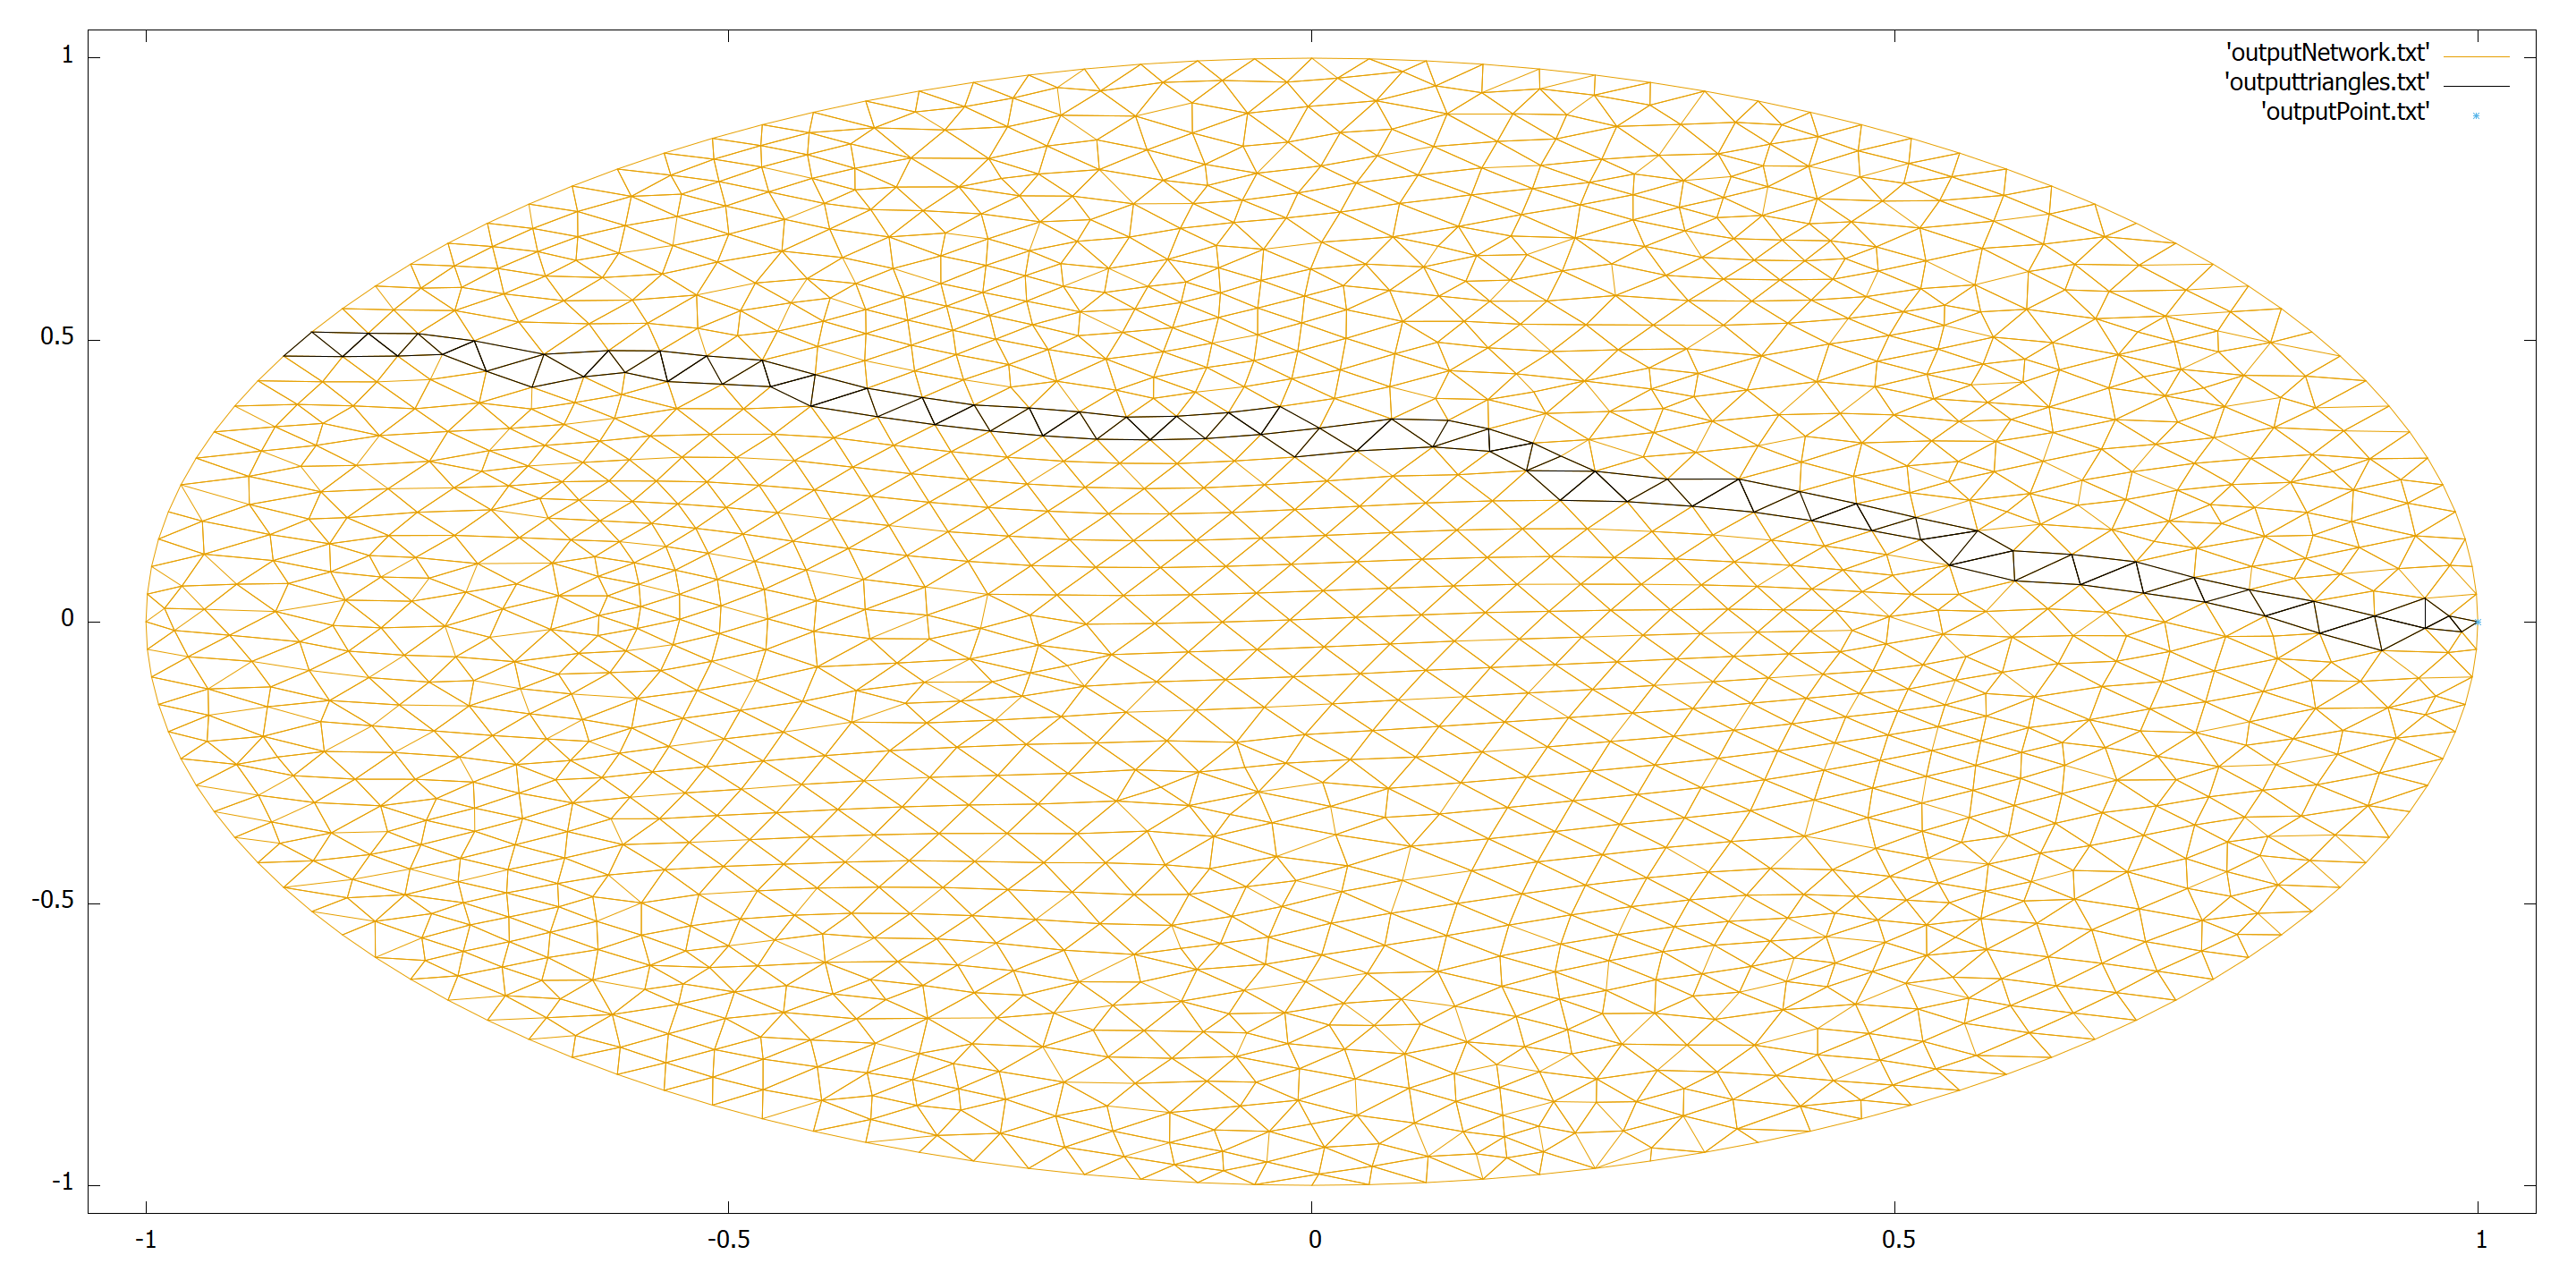
\includegraphics[width=0.55\linewidth, height=0.55\linewidth]{../Figures/StartTri600_p(1,0)_min_neg}}
%	\caption{}
	\subfigure{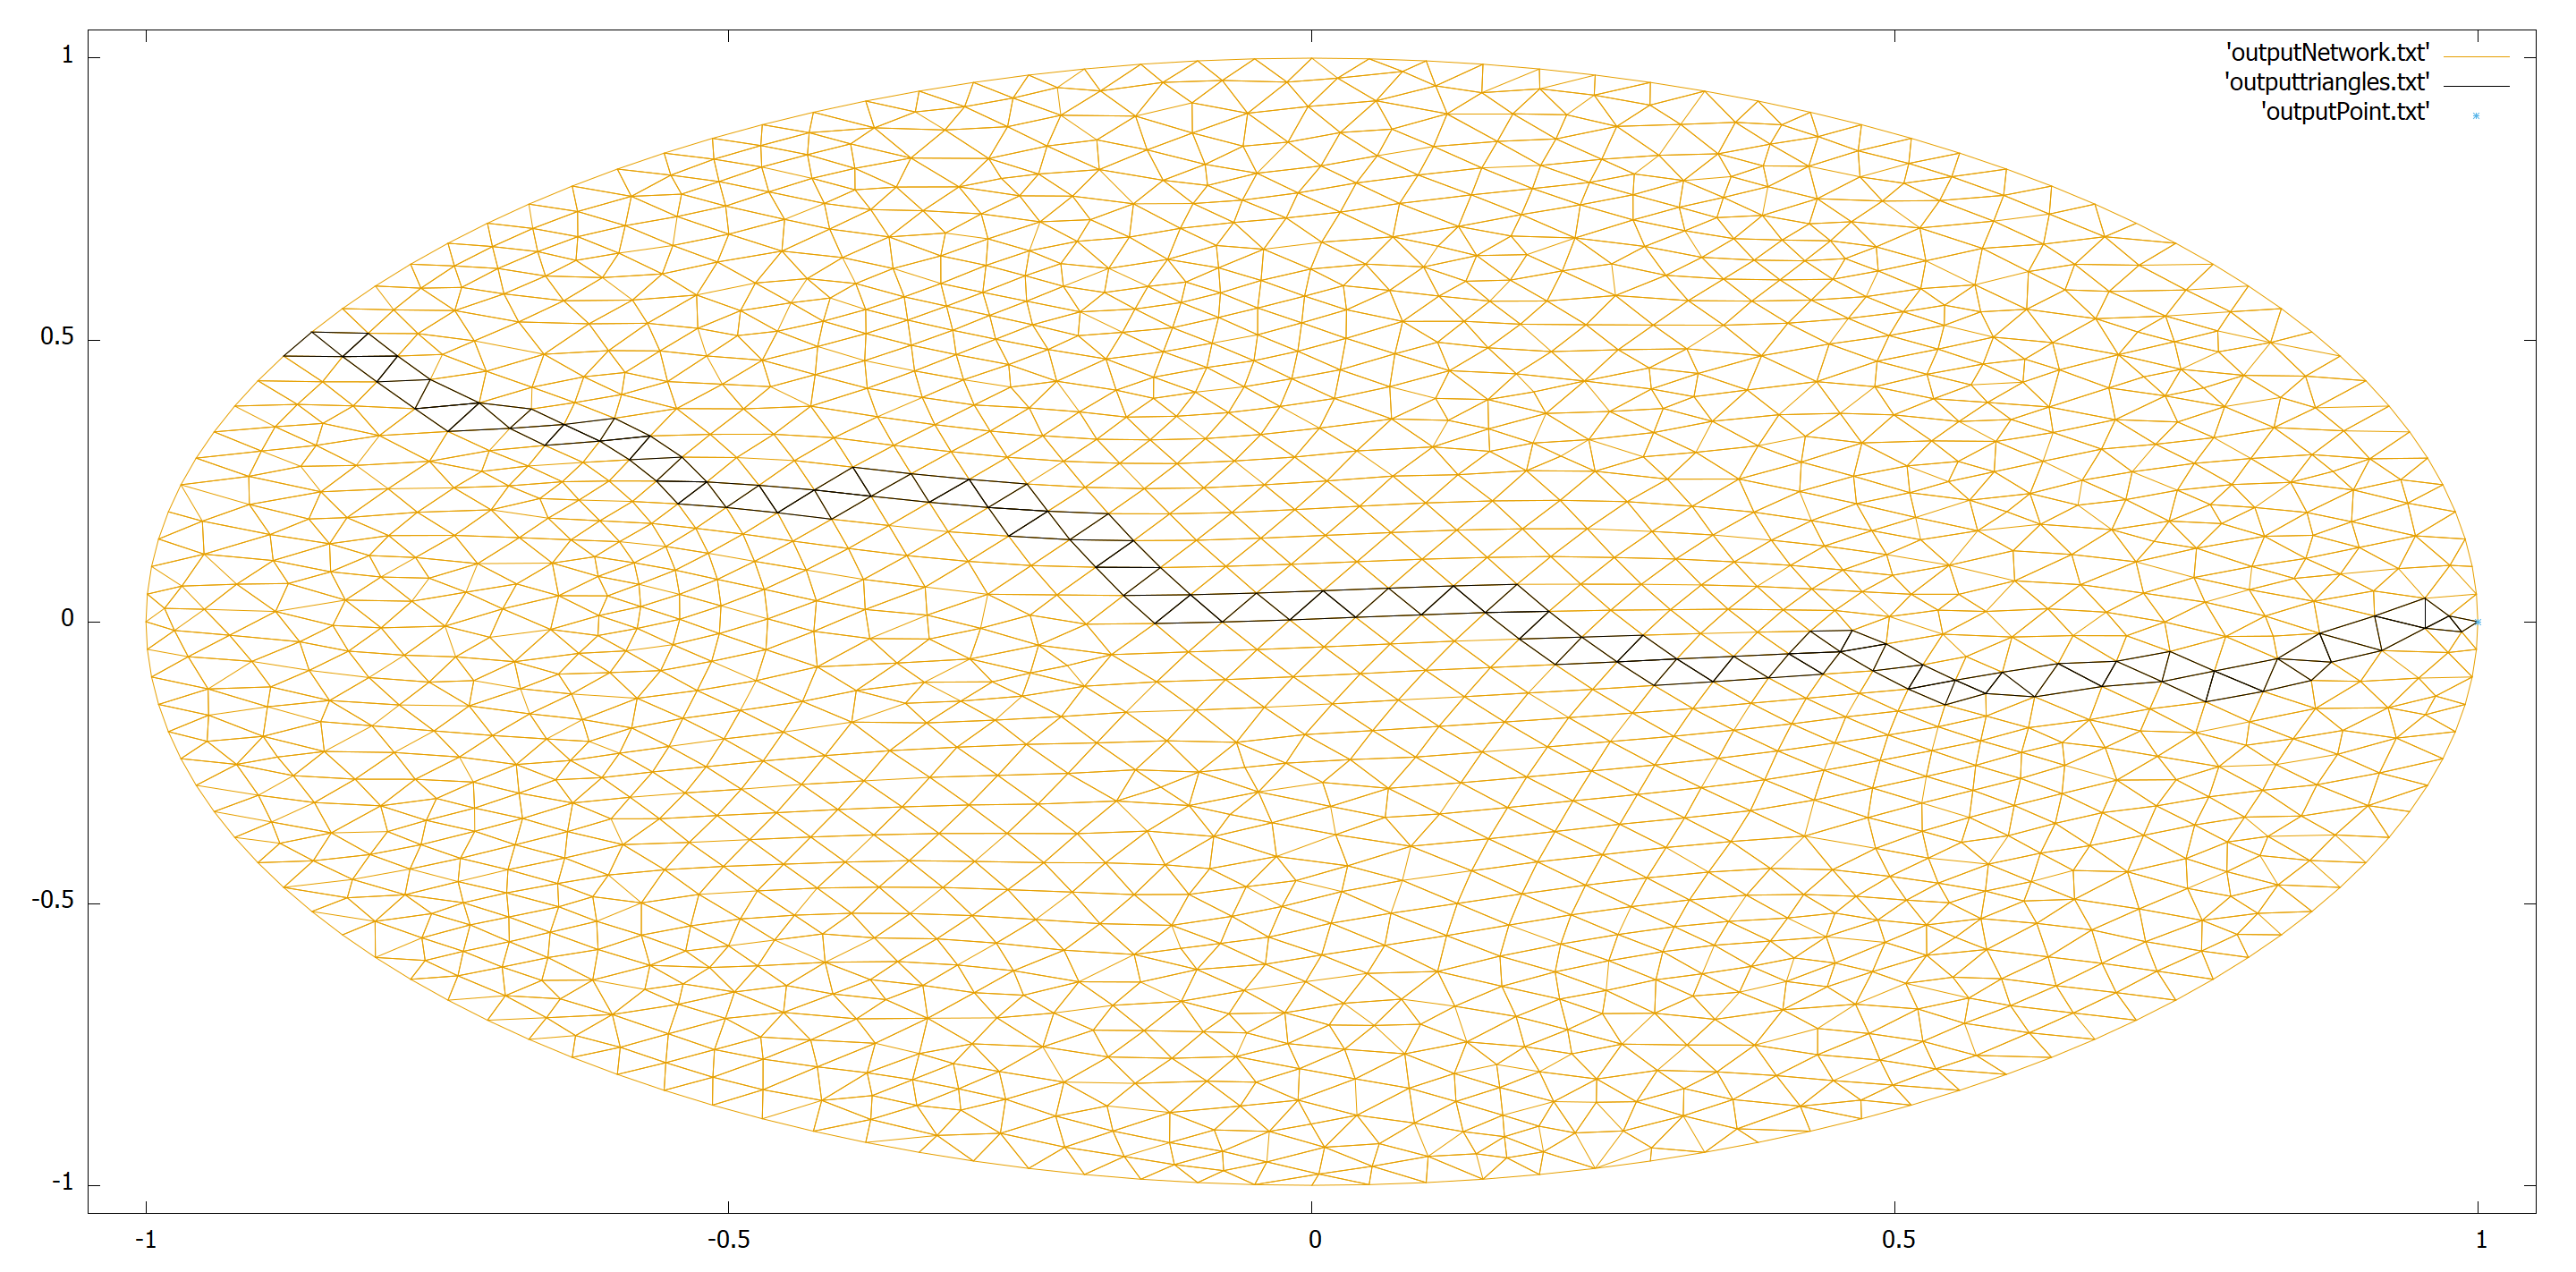
\includegraphics[width=0.55\linewidth,height=0.55\linewidth]{../Figures/StartTri600_p(1,0)_random_neg1}}
\end{figure}

\begin{figure}[h]
	\subfigure{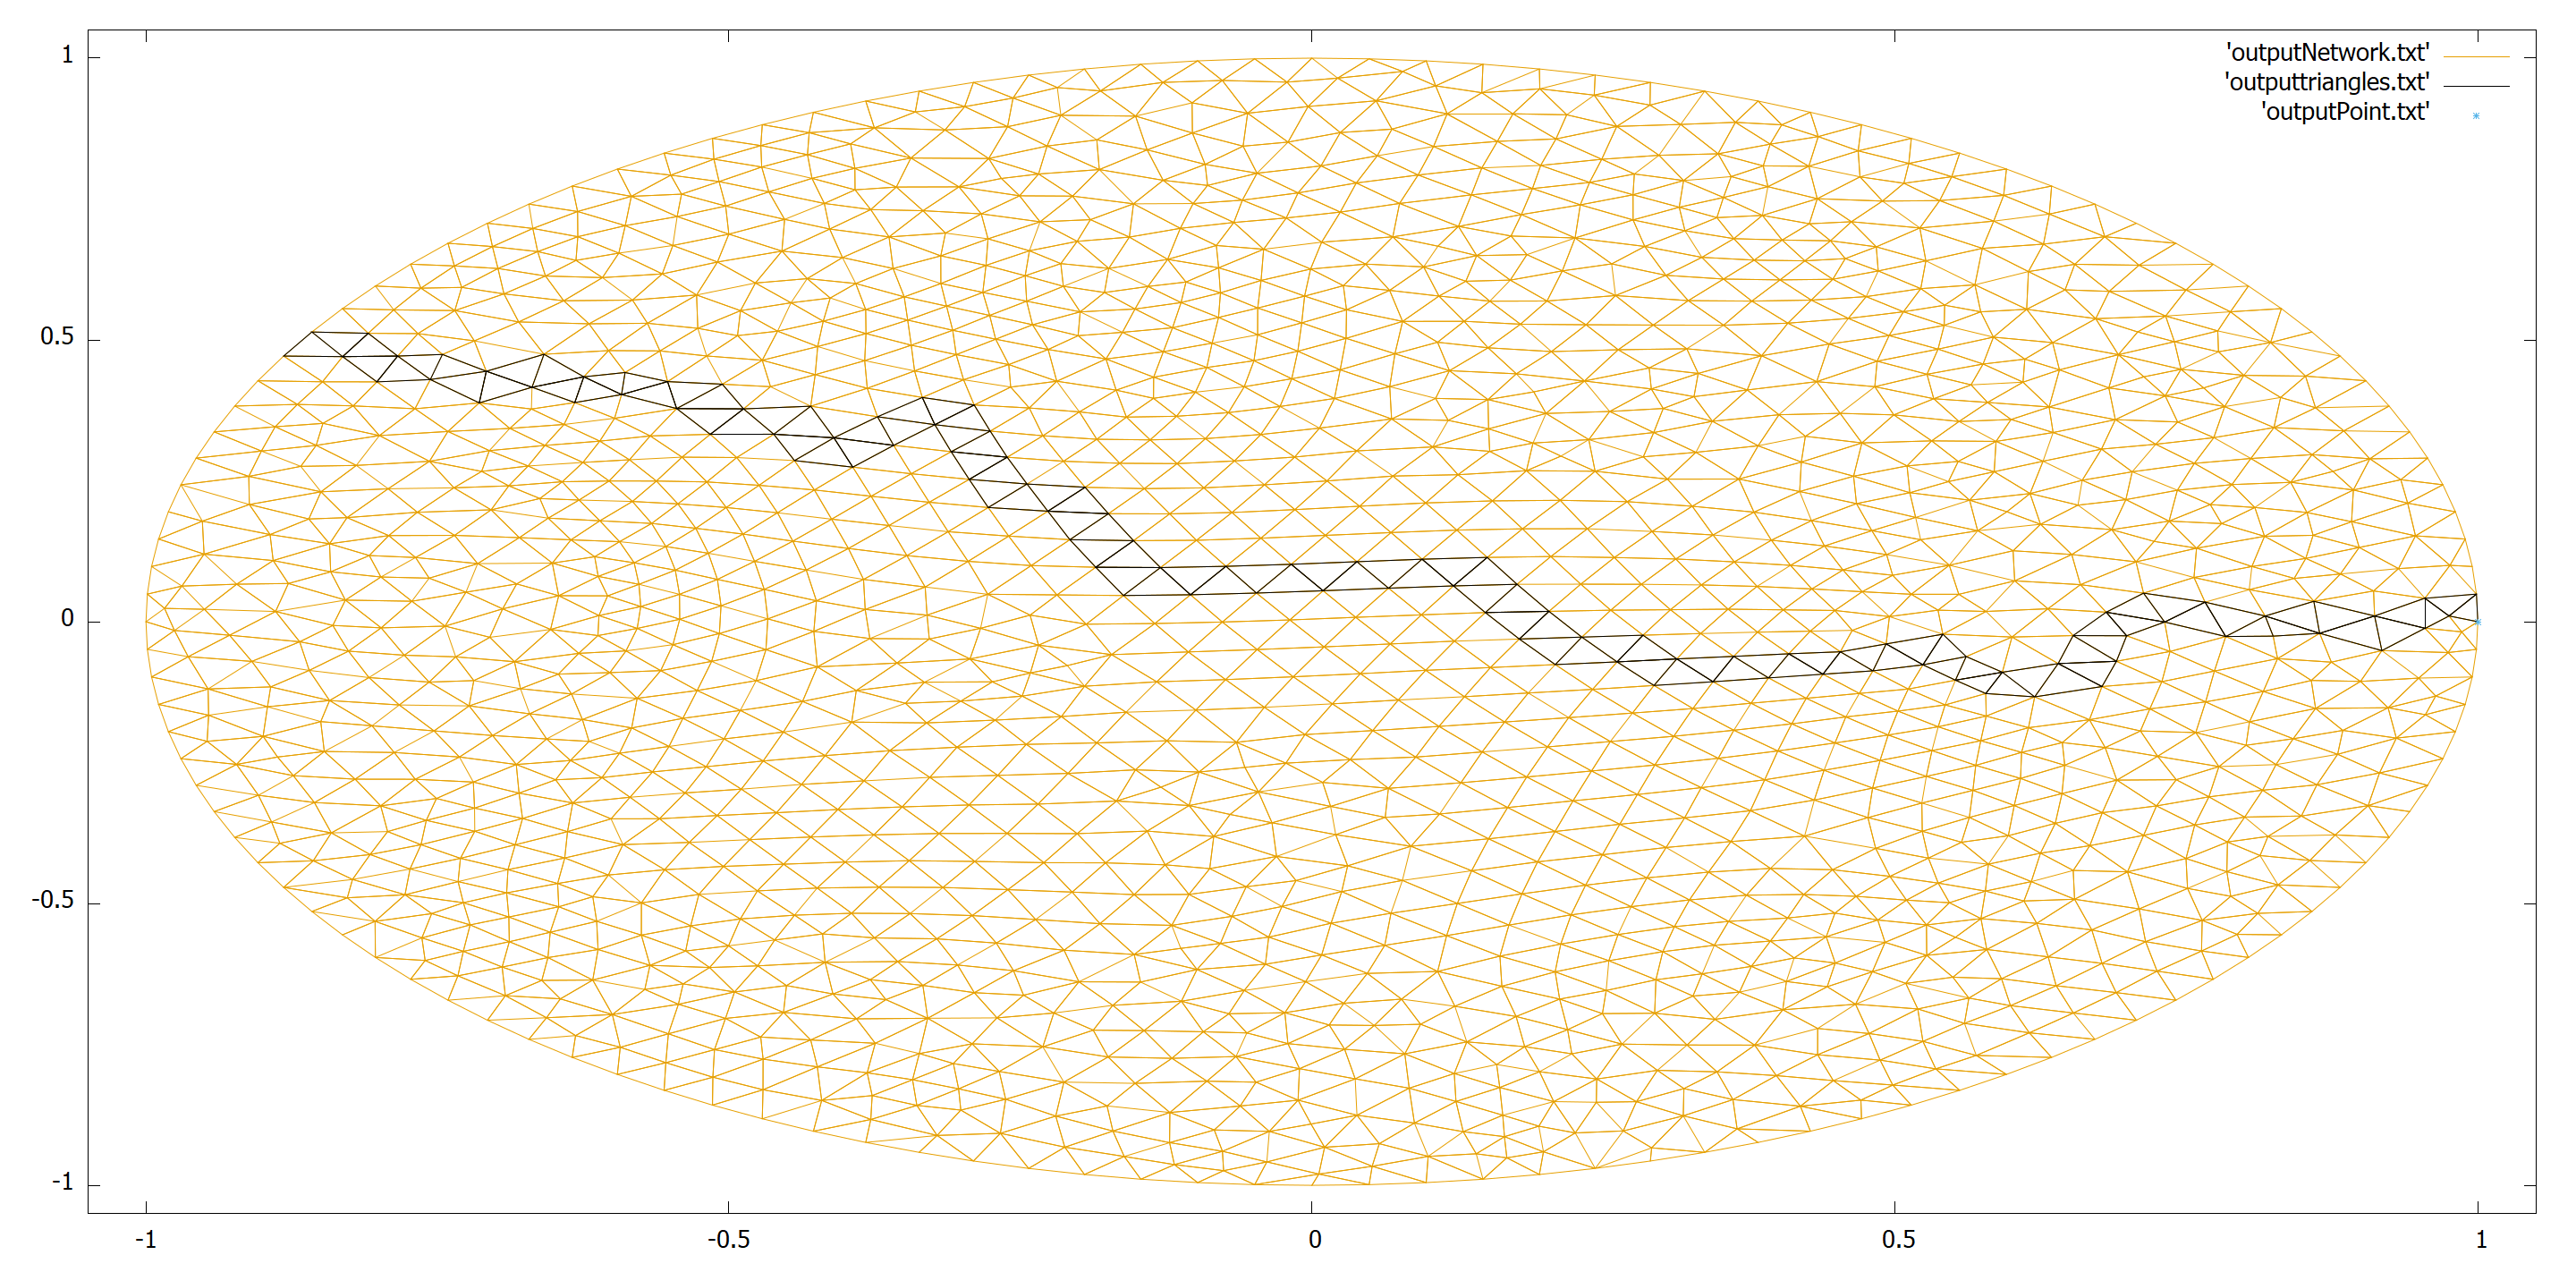
\includegraphics[width=0.55\linewidth,height=0.55\linewidth]{../Figures/StartTri600_p(1,0)_random_neg2}}
	\subfigure{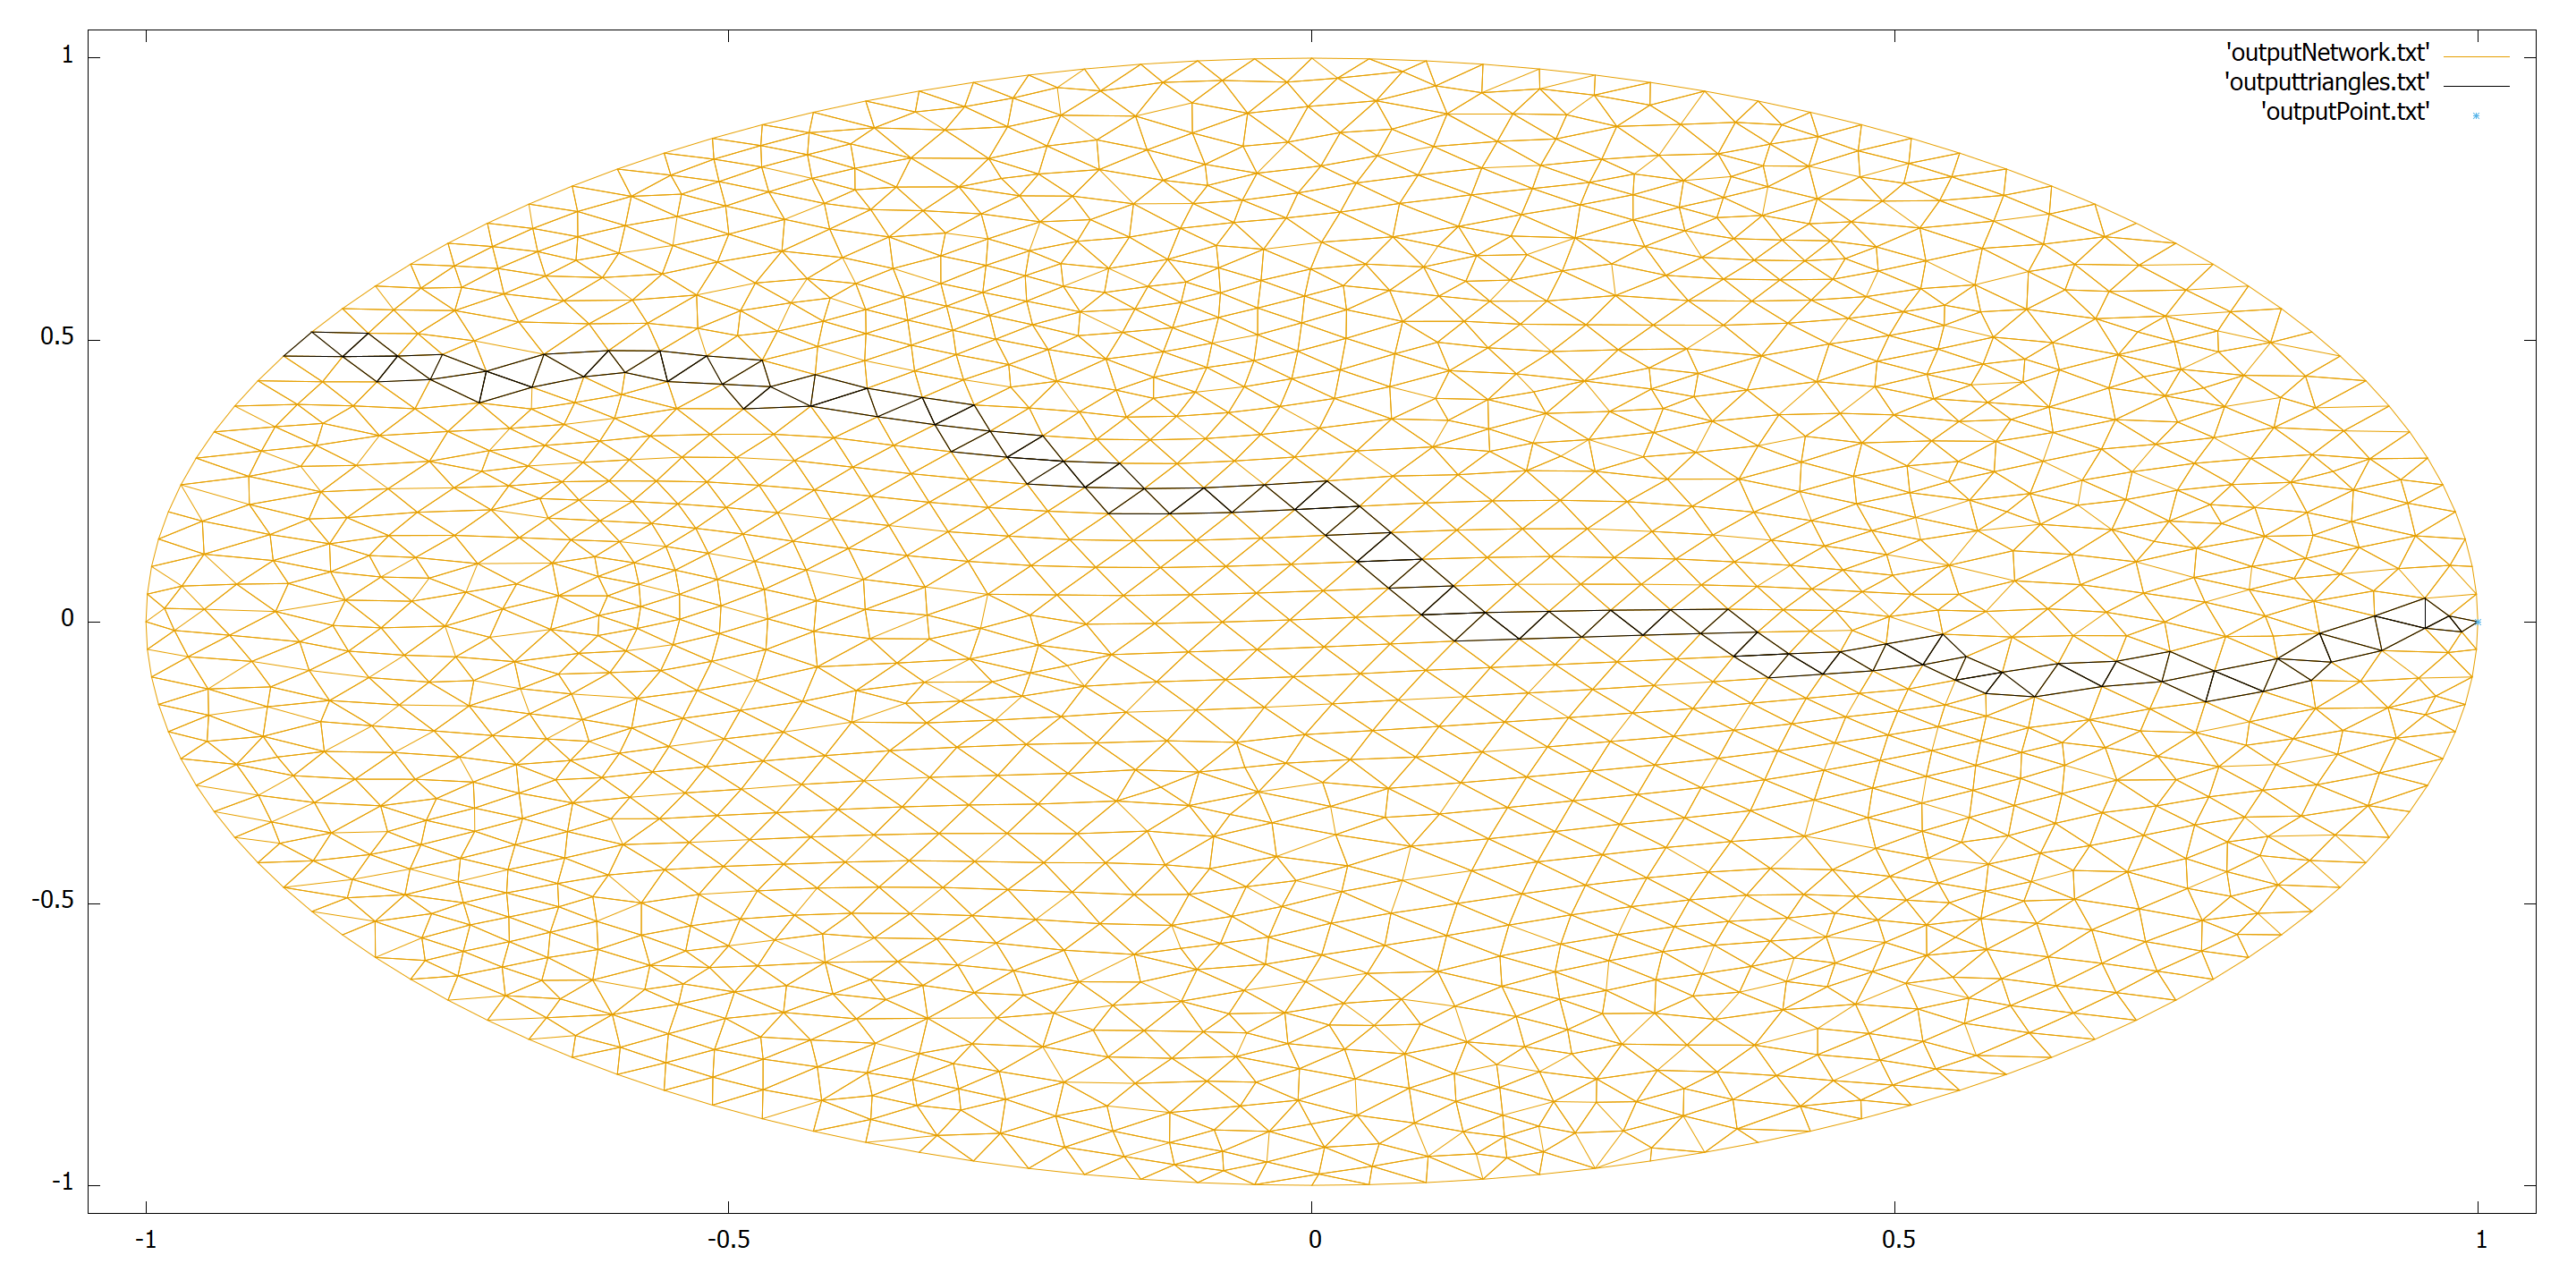
\includegraphics[width=0.55\linewidth,height=0.55\linewidth]{../Figures/StartTri600_p(1,0)_random_neg3}}
\end{figure}

\begin{figure}[h]  \label{ex}

		\subfigure{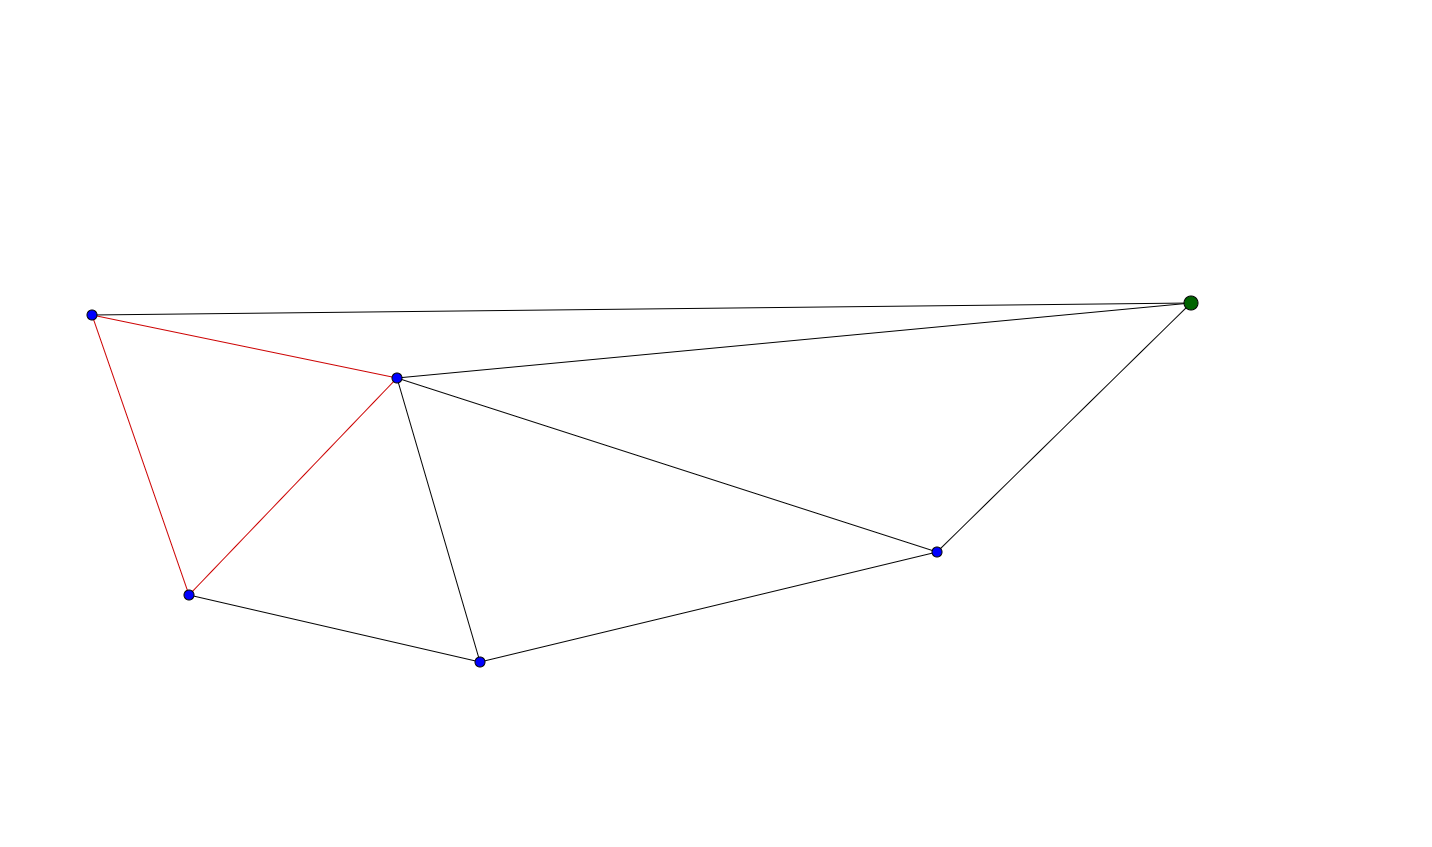
\includegraphics[width=0.55\linewidth,height=0.55\linewidth]{ExampleMaillage.png}}
		\caption{An example of a mesh where a random choice of the consecutive triangle is better.}
		\subfigure{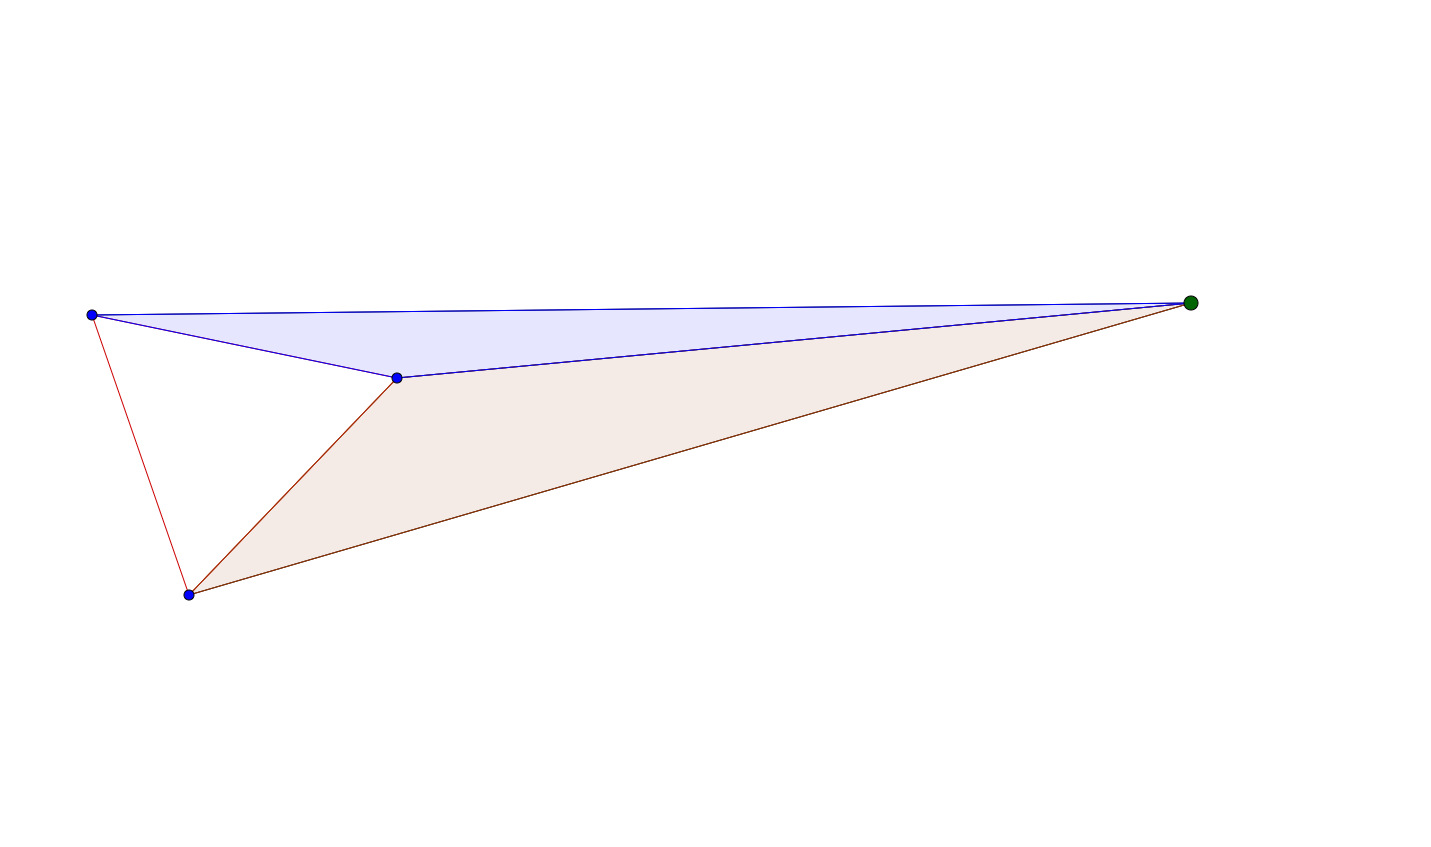
\includegraphics[width=0.55\linewidth,height=0.55\linewidth]{ExampleComparisaon.png}}
		\caption{If the choice of the next triangle is not random it is determined according to the size of the blue and red surfaces.  }
	

	
\end{figure}
As shown in figure \ref{ex} a random choice of the following triangle can be better. If the algorithm starts with the red triangle and is searching for the green point it has to decide if it takes the neighbor lying relatively higher in the plane or the one lying relatively lower. Deciding this by the smaller oriented volume the lower one will be chosen. 

\subsection{The visualization via gnuplot}
	The visualization is done by the function $ exportGnuplot $ being able to visualize two different things: 
	\begin{enumerate}
		\item 
		The result of the algorithm promenade, that is a sequence of adjacent triangles from a starting triangle to a triangle covering the searched point. 
		In this case the input variable $ triangles_path $ contains the sequence of triangles and the input variable $  points $ contains just one point, hence the input $ int numbpoints $ is $ 1 $. 
		\item 
		Given a mesh and the points of another mesh it can visualize the set of the covering triangles (a subset of triangles of the first mesh) of the points of the second mesh. 
		In this case the input variable $ tirangles_path $ contains the covering triangles and the $ points $ are the points of the second mesh. 
	\end{enumerate}
The functions writes four text files, one for all triangles of the mesh, one for the triangles in $ triangles_path $, one for the points in $ points $ and one for the commands which shall be executed by gnuplot. This is all realized by a simple $ ofstream $ variable, allowing to create and manipulate a text file. //
The script for gnuplot contains a line which keeps the plot open until some key is hit in the terminal. 
The actual execution in the terminal is achieved by the command $ system $ which executes its input string in the terminal. 

\section{5 find covering Triangles}

\section{Testumgebung - main}

\end{document}





